\section{Simple distributed image reconstruction}\label{dist}
Distribute the major cycle we need several major cycle iterations. We cannot execute the second cycle before the first. So we need to distribute the steps in the major cycle, namely the gridding, FFT and deconvolution step. 

Gridding is generally the most time intensive step. 
Large number of visibilities, forces us to partition the input data. Meaning each node has only part of the data. This work assumes we have a copy of the full grid on each node. and exchange
We use the Image Domain Gridding algorithm.

The FFT is generally not worth distributing, if we can keep all the data in memory. When the gridding is done, in our setup, the grid is small enough to keep in memory.

Deconvolution is potentially the second most time consuming step after the Gridding.
Depends on the image content.
Deconvolution produces the model image and the residual image.
Distributed deconvolution requires communication. How we communicate is key.
Distributing the deconvolution generally leaves us with two possible architectures: Either we split the deconvolution problem into patches, or we create a consensus algorithm. Consensus algorithms work by each node having a copy of the model image, and as a group, decide on the equal image. Not very useful for Meerkat, since we potentially do the work several times. 
We then want to distribute the work as evenly as possible between the nodes. 
That is why we chose to split the data onto nodes. 


This leads us to the following architecture.
\begin{figure}[h]
	\centering
	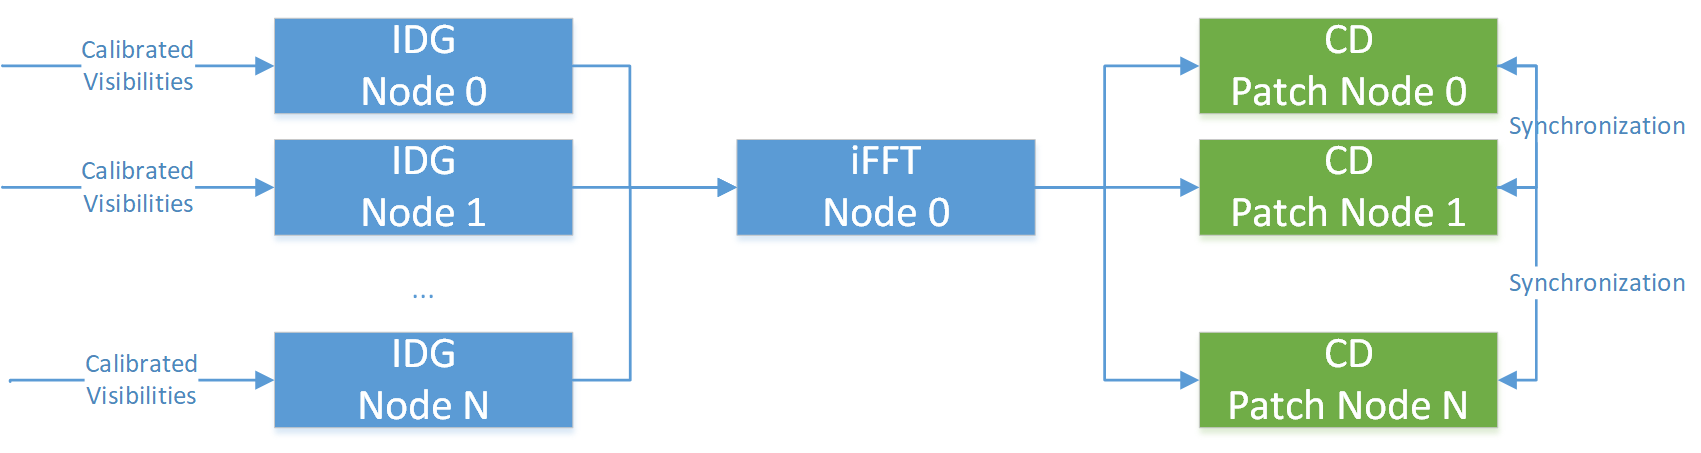
\includegraphics[width=0.80\linewidth]{./chapters/03.distribution/distributed_architecture.png}
	\caption{Distributed architecture for half a major cycle}
	\label{dist:architecture:fig}
\end{figure}

Rest of the Major Cycle. We need to get the model image patches from the nodes, FFT on node 0, and then we communicate the grid.


\subsection{Distributing the IDG Algorithm}\label{distribution:idg}
It is simple, unlike $w$-stacking, we do not need to partition the data. So we can do just communicate the grid



\subsection{Distributed deconvolution algorithm}

Coordinate Descent Algorithm why.

Basic algorithm.


Implementation
Correlate the dirty image
Find max
How to calculate a

\subsubsection{ElasticNet Regularization}
L2 norm was used in other work. \cite{Ferrari}


Formula

\begin{figure}[h]
	\centering
	\begin{subfigure}[b]{0.3\linewidth}
		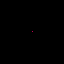
\includegraphics[width=\linewidth]{./chapters/03.distribution/L1.png}
		\caption{Effect of the pure L1 norm ($\lambda$ = 1.0) on a single point source.}
		\label{dist:cd:elastic:L1}
	\end{subfigure}
	\begin{subfigure}[b]{0.3\linewidth}
		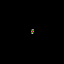
\includegraphics[width=\linewidth]{./chapters/03.distribution/L2.png}
		\caption{Effect of the pure L2 norm ($\lambda$ = 1.0) on a single point source.}
		\label{dist:cd:elastic:L2}
	\end{subfigure}
	
	\caption{Effect of the L1 and L2 Norm separately.}
	\label{dist:cd:elastic}
\end{figure}


Effect

Implementation



May even speed up convergence for correlated pixel values compared to L1 or L2\cite{friedman2010regularization}. But was not investigated in this project

\subsection{Major Cycle convergence}
Putting it all together

We have the Minor Cycle, which is easy to converge.

Coordinate Descent Path optimization \cite{friedman2010regularization}
Danger that CD takes too many pixel into a Major Cycle. Lower bound per iteration, PSF sidelobe
  can still be too low, danger when many psf sidelobes overlap

\subsection{Test on MeerKAT data}

